This chapter details the implementation of the automated solution proposed in Chapter \ref{chap:context}. First, an overview of the various components implemented throughout the project is given. Next, the implementation of a deep network capable of automatically extracting annual density bands present in two dimensional data is discussed. The attempts at implementing a network capable of automatically extracting the annual density bands present in three dimensions are also detailed. Then, the implementation of and reasoning behind the custom accuracy metric are discussed. Finally, the techniques used to estimate the calcification rate from the extracted boundaries are described.

\section{Overview}

A system capable of calculating of the calcification rate given only some section of density data requires the implementation of many separate subcomponents. The diagram below provides an overview of these components and outlines the order in which they were implemented and will be discussed.

\includegraphics[width=\textwidth, height=0.74\textwidth]{example-image-a}

\section{Two Dimensional Boundary Extraction}

This section outlines the steps taken to implement and train a CNN capable of extracting the annual density banding present in two dimensional data.

\subsection{Labelling the Data}

In order for a supervised CNN to perform well, large amounts of labelled data much be available to train on. Since the dataset provided was initially unlabelled, a manual labelling process was devised and is described in this section.

\subsubsection{The Initial Dataset}

The dataset provided contains more than 160 three dimensional computed tomography (CT) scans of unique coral skeletons from the Natural History Museum's collection. Each individual 3D scan consists of stacks of thousands of 2D \texttt{.tif} images which will be referred to as ``slices''. This unlabelled dataset will be referred to as the ``initial dataset''. Although the initial dataset contains scans of ten different genera of coral, only scans of the Porites genus were considered for labelling and training the network with. An example of a Porites skeleton that is part of the dataset is shown in Figure \ref{fig:scanexample}. The Porites scans were chosen as they contain annual banding that can be more easily identified and labelled.

A typical scan consists of ${\sim}2000$ slices that each have the same resolution of typically ${\sim}$2000$\times$2000 pixels resulting in an overall 3D resolution of 2000$\times$2000$\times$2000 voxels. The 3D resolution of each scan varies, but the scale (e.g., the number of voxels used to represent a centimetre cubed) is consistent across scans.

\begin{figure}[t]
    \centering
    \begin{subfigure}[t]{0.49\textwidth}
        \centering
        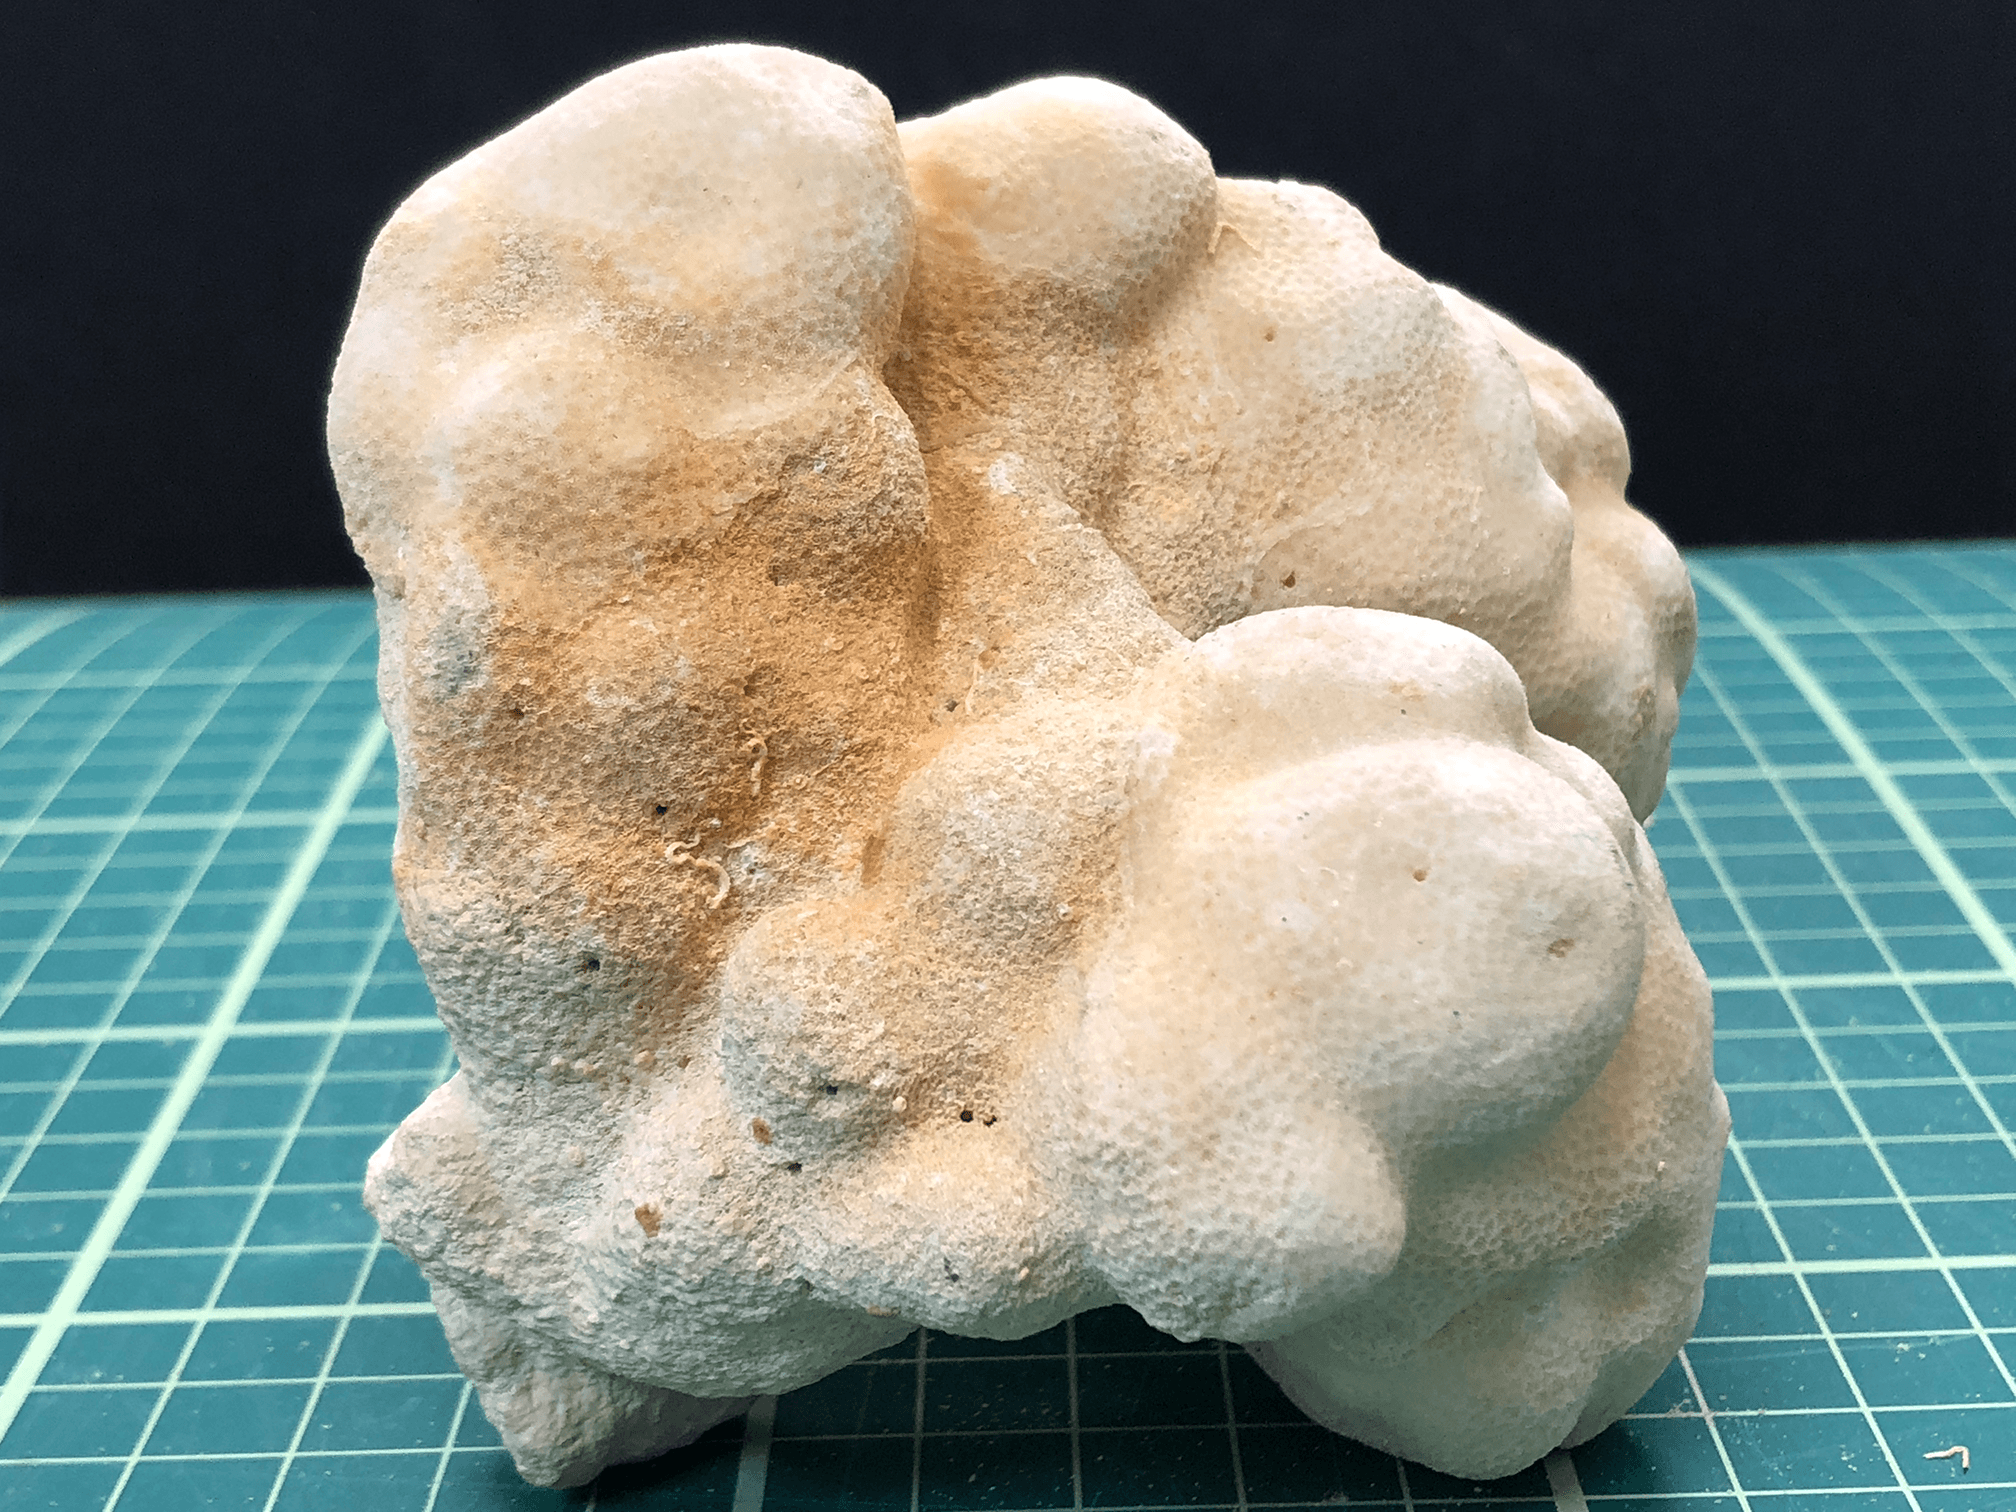
\includegraphics[width=1\textwidth, valign=c]{images/real-coral.png}
    \end{subfigure}
    ~
    \begin{subfigure}[t]{0.49\textwidth}
        \centering
        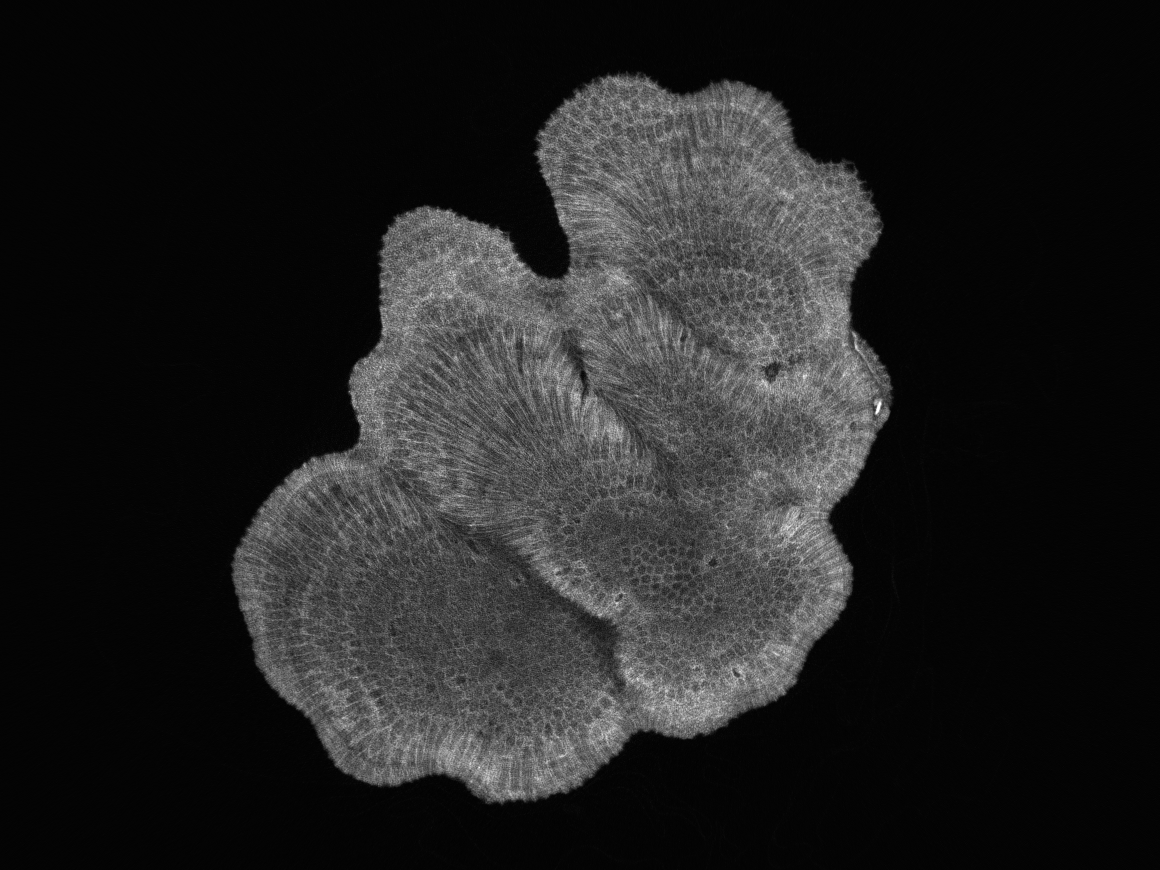
\includegraphics[width=1\textwidth, valign=c]{images/slice-example.png}
    \end{subfigure}
    \caption{\textbf{(left)} An example of a Porites coral skeleton from the Natural History Museum's collection. This particular sample was collected from the Solomon Islands in 1974. In the initial dataset, the scan of this sample is represented by 1945$\times$1508$\times$1208 voxels. \textbf{(right)} A 2D slice extracted from the CT scan of the sample shown on the left. The slice is a negative; brighter pixels correspond to high density and darker pixels correspond to low density.}
    \label{fig:scanexample}
\end{figure}

\subsubsection{Slice Selection and Extraction}

Not all slices that compose a scan contain annual density banding that can confidently be identified. In order to find appropriate slices, each Porites scan was opened and inspected manually using a 3D visualisation program called Avizo\footnote{\url{https://tiny.cc/avizo}}. Avizo allows users to view slices orthogonal to the $x$, $y$, or $z$ axis of a scan. A selection of seven slices that could confidently be labelled were chosen. Once these slices were identified, a Python script was used to extract each slice and export them as greyscale PNG images. The slices can be represented as greyscale images since they only require one channel to represent depth. Some of the adjacent slices were also extracted in order to curate the 3D dataset used later in the project (discussed in Section~\ref{sec:threedimension}).

\subsubsection{Slice Labelling}

Once the slices were selected, a labelling process was established. Initially, two methods of labelling were considered and shown to Dr Erica Hendy, a senior lecturer in biogeochemical cycles. Of the two methods (shown in Figure \ref{fig:labelstyle}), the ``smooth'' method was deemed as the more realistic choice. An idealised annual density cycle is actually in the form of a sinusoidal wave with the density gradually changing from high to low and back over the course of a year~\cite[p. 39]{coralsine}. Thus, an exact boundary between a high and low band does not actually exist, making the ``complex'' method unrealistic both in terms of reproducibility, and in terms of biological accuracy.

\begin{figure}[t]
    \centering
    \begin{subfigure}[t]{0.49\textwidth}
        \centering
        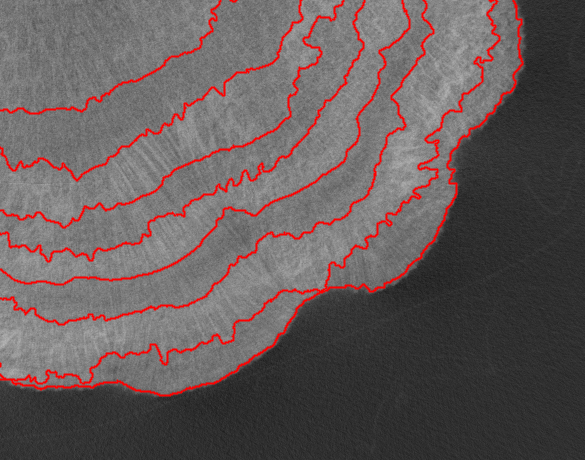
\includegraphics[width=1\textwidth, valign=c]{images/rough-label.png}
    \end{subfigure}
    ~
    \begin{subfigure}[t]{0.49\textwidth}
        \centering
        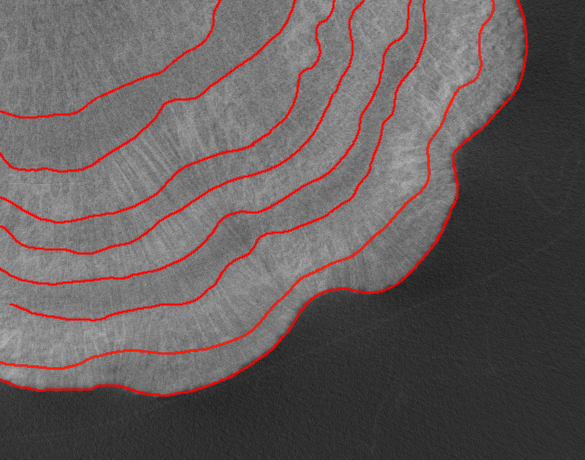
\includegraphics[width=1\textwidth, valign=c]{images/smooth-label.png}
    \end{subfigure}
    \caption{A comparison of the two methods of labelling that were initially considered. The boundary labels are coloured red and placed over the the same original negative 2D slice. \textbf{(left)} A method of labelling in which the boundaries were placed on the sharpest change in density resulting in complex boundaries whose positions are highly sensitive to noise in the image. \textbf{(right)} A method in which the chosen boundaries are ``smooth'' whilst also being placed as close as possible to the sharpest change in density.}
    \label{fig:labelstyle}
\end{figure}

Each selected slice was then manually labelled using the GNU Image Manipulation Program (GIMP)\footnote{\url{https://www.gimp.org}}. A one pixel wide white line is drawn at the beginning and end of each annual high density band and the rest of the image is black---no values other than black or white are present in the labels. In order to ensure that the decisions made regarding the boundaries of the annual bands were as consistent as possible, each slice was manually labelled three or more times, and the most common boundaries were chosen. It is important for the labelling method to be consistent and reproducible as this enables the dataset to be expanded in the future.

\subsection{Dataset Curation}

Since only Once the slices had been manually selected and labelled, a dataset of 

In order for a supervised CNN to perform well, large amounts of labelled data much be available to train on. Since the dataset provided was initially unlabelled, a manual labelling process was devised and is described in this section.

\subsubsection{Sliding Window}

show snippet of the code used for sliding window.

show table of number of produced slices from each sample

Multiple slices from each of the four chosen scans were labelled. Each slice was then used to produce ${\sim}$50 -- 200 samples using a sliding-window technique with a stride of 20 pixels. The number of samples produced per slice depended on how large the confidently labelled area was, since often only sections of a slice display identifiable annual banding. The corresponding labels for each sample were also produced. The resulting samples and labels were 224$\times$224 greyscale PNG images. In total, 524 samples were produced. These samples and their corresponding labels were then used to train the network.

\begin{table}[t]
\centering
\caption{A table showing the... blah blah blah}
\begin{tabular}{@{}lrrrrrr@{}}
\toprule
Slice & $x_{top}$ & $y_{top}$ & $x_{bottom}$ & $y_{bottom}$ & Stride (px) & Patches produced \\ \midrule
RS0030\_yz\_0625.tif    & 1028      & 153       & 1350         & 530          & 20          & 36      \\
RS0030\_yz\_0642.tif    & 1070      & 143       & 1390         & 463          & 20          & 18      \\
RS0030\_yz\_0642.tif    & 895       & 400       & 1275         & 685          & 20          & 12      \\
RS0116\_0414.tif        & 666       & 1258      & 1560         & 1750         & 40          & 150     \\
RS0116\_0500.tif        & 970       & 1320      & 1320         & 1854         & 30          & 54      \\
RS0116\_0500.tif        & 1130      & 1250      & 1525         & 1730         & 30          & 56      \\
RS0128\_yz\_0451.tif    & 490       & 258       & 790          & 690          & 20          & 32      \\
RS0130\_xz\_0820.tif    & 513       & 1190      & 828          & 1485         & 10          & 30      \\ \midrule
Total                   &           &           &              &              &             & 388     \\ \bottomrule
\end{tabular}
\end{table}

\subsubsection{Splitting the Dataset}

talk about rationale behind the splits

\subsection{Data Augmentation}

\subsection{Architecture}

Implementation of architecture

Spatial drop out better for fully conv? \url{https://arxiv.org/pdf/1411.4280.pdf}

% From Keras docs I think
% This version performs the same function as Dropout, however it drops
% entire 2D feature maps instead of individual elements. If adjacent pixels
% within feature maps are strongly correlated (as is normally the case in
% early convolution layers) then regular dropout will not regularize the
% activations and will otherwise just result in an effective learning rate
% decrease. In this case, SpatialDropout2D will help promote independence
% between feature maps and should be used instead.

\subsection{Early Stopping and Checkpointing}

\section{Three Dimensional Boundary Extraction}
\label{sec:threedimension}

This section discusses the attempts to implement and train a CNN capable of extracting the annual density banding present in three dimensional data.

\subsection{Dataset Expansion}

\subsection{Architecture Modification}

\subsection{Data Loader Implementation}

\subsection{Three Dimensional Data Augmentation}

\section{Accuracy Metric Implementation}

\subsection{Skeletonisation}

(Show algorithm and maybe some source code?)

\subsection{The \texttt{ctypes} Module}

\section{Density Band Width Estimation}

\subsection{Point Sampling}

% {\bf A topic-specific chapter, of roughly $15$ pages} 
% \vspace{1cm} 

% \noindent
% This chapter is intended to describe what you did: the goal is to explain
% the main activity or activities, of any type, which constituted your work 
% during the project.  The content is highly topic-specific, but for many 
% projects it will make sense to split the chapter into two sections: one 
% will discuss the design of something (e.g., some hardware or software, or 
% an algorithm, or experiment), including any rationale or decisions made, 
% and the other will discuss how this design was realised via some form of 
% implementation.  

% This is, of course, far from ideal for {\em many} project topics.  Some
% situations which clearly require a different approach include:

% \begin{itemize}
% \item In a project where asymptotic analysis of some algorithm is the goal,
%       there is no real ``design and implementation'' in a traditional sense
%       even though the activity of analysis is clearly within the remit of
%       this chapter.
% \item In a project where analysis of some results is as major, or a more
%       major goal than the implementation that produced them, it might be
%       sensible to merge this chapter with the next one: the main activity 
%       is such that discussion of the results cannot be viewed separately.
% \end{itemize}

% \noindent
% Note that it is common to include evidence of ``best practice'' project 
% management (e.g., use of version control, choice of programming language 
% and so on).  Rather than simply a rote list, make sure any such content 
% is useful and/or informative in some way: for example, if there was a 
% decision to be made then explain the trade-offs and implications 
% involved.

% \section{Example Section}

% This is an example section; 
% the following content is auto-generated dummy text.
% \lipsum

% \subsection{Example Sub-section}

% \begin{figure}[t]
% \centering
% foo
% \caption{This is an example figure.}
% \label{fig}
% \end{figure}

% \begin{table}[t]
% \centering
% \begin{tabular}{|cc|c|}
% \hline
% foo      & bar      & baz      \\
% \hline
% $0     $ & $0     $ & $0     $ \\
% $1     $ & $1     $ & $1     $ \\
% $\vdots$ & $\vdots$ & $\vdots$ \\
% $9     $ & $9     $ & $9     $ \\
% \hline
% \end{tabular}
% \caption{This is an example table.}
% \label{tab}
% \end{table}

% \begin{algorithm}[t]
% \For{$i=0$ {\bf upto} $n$}{
%   $t_i \leftarrow 0$\;
% }
% \caption{This is an example algorithm.}
% \label{alg}
% \end{algorithm}

% \begin{lstlisting}[float={t},caption={This is an example listing.},label={lst},language=C]
% for( i = 0; i < n; i++ ) {
%   t[ i ] = 0;
% }
% \end{lstlisting}

% This is an example sub-section;
% the following content is auto-generated dummy text.
% Notice the examples in Figure~\ref{fig}, Table~\ref{tab}, Algorithm~\ref{alg}
% and Listing~\ref{lst}.
% \lipsum

% \subsubsection{Example Sub-sub-section}

% This is an example sub-sub-section;
% the following content is auto-generated dummy text.
% \lipsum

% \paragraph{Example paragraph.}

% This is an example paragraph; note the trailing full-stop in the title,
% which is intended to ensure it does not run into the text.
